\chapter{Production of word-final /s/}\label{chapter04}

As explained in detail in Section \ref{section02_1}, the present production study investigates the potential durational differences between three types of word-final /s/: non-morphemic /s/, plural /s/, and clitic /s/ (with the auxiliaries \textit{is} and \textit{has}).\footnote{An earlier version of this chapter has been published as part of \citet{Schmitz2021a}.} Pseudowords are used as items to prevent potential lexical effects to confound findings (see Section \ref{section03_1_1}). Three hypotheses derived from theories and models of speech production are examined. \textsc{H prod\textsubscript{1}}, the ``Feed-Forward Hypothesis", assumes that there is no durational difference between different types of word-final /s/. According to \textsc{H prod\textsubscript{2}}, the ``Prosodic Hypothesis", non-morphemic /s/ is shorter than plural /s/, and plural /s/ is shorter than auxiliary clitic /s/. \textsc{H prod\textsubscript{3}}, the ``Emergence Hypothesis", assumes that there are durational differences between different types of word-final /s/, but does not indicate what the nature of these durational differences is.

\section{Methodology}\label{section04_1}

\subsection{Speakers and recordings}\label{section04_1_1}

Forty native speakers of Southern British English took part in the experiment. Their mean age was 28.7 years, ranging from 19 to 58. Eight speakers were bi- or multilingual, and twenty-five speakers were from London while the other fifteen speakers were from other places in South Britain. None of the participants had a background in linguistics.

The recordings took place at Chandler House, University College London. The acoustic data were recorded on a computer with a Røde NT1-A microphone using an RME Fireface UC audio interface and sampled at 44.1 kHz, 16 bit.

\subsection{Materials}\label{section04_1_2}

For the production experiment, the pseudoword paradigm by \citet{Berko1958} was adopted. Following her reasoning, it was assumed that phonetic effects found in pseudoword paradigms mirror linguistic reality. The pseudowords used in the production experiment consist of the full set of pseudowords discussed in detail in Section \ref{section03_1_2}. For reasons of convenience, Table \ref{tab:4.1} lists these pseudowords once more.

\begin{table}\fontsize{10}{11}
\caption{Orthographic representations of all pseudowords.}
\label{tab:4.1}
\centering
\begin{tabular}{cccccc} 
\lsptoprule
gli-           & pru-           & plee-           & cloo-           & blou-           & glai-            \\ 
\midrule
\textit{glip}  & \textit{prup}  & \textit{pleep}  & \textit{cloop}  & \textit{bloup}  & \textit{glaip}   \\
\textit{glit}  & \textit{prut}  & \textit{pleet}  & \textit{cloot}  & \textit{blout}  & \textit{glait}   \\
\textit{glik}  & \textit{pruk}  & \textit{pleek}  & \textit{clook}  & \textit{blouk}  & \textit{glaik}   \\
\textit{glif}  & \textit{pruf}  & \textit{pleef}  & \textit{cloof}  & \textit{blouf}  & \textit{glaif}   \\ 
\midrule
\textit{glips} & \textit{prups} & \textit{pleeps} & \textit{cloops} & \textit{bloups} & \textit{glaips}  \\
\textit{glits} & \textit{pruts} & \textit{pleets} & \textit{cloots} & \textit{blouts} & \textit{glaits}  \\
\textit{gliks} & \textit{pruks} & \textit{pleeks} & \textit{clooks} & \textit{blouks} & \textit{glaiks}  \\
\textit{glifs} & \textit{prufs} & \textit{pleefs} & \textit{cloofs} & \textit{bloufs} & \textit{glaifs}  \\
\lspbottomrule
\end{tabular}
\end{table}

To elicit the pertinent types of /s/ under investigation, i.e. non-morphemic, plural, and \textit{is}- and \textit{has}-clitic /s/, 48 contexts and accompanying questions for /s/ elicitation were created. The verbs directly following the pseudowords in these contexts were chosen in such a way that out of twelve verbs in total, three each started with a voiceless plosive (/pl/, /k/), a vowel (/ɑ/, /i:/, /ʌ/, /eɪ/), a nasal (/m/, /n/), and an approximant (/w/, /l/, /r/). This was done to control for possible coarticulatory effects of these segmental classes with the preceding /s/. Examples are given in \ref{ex:4.1} to \ref{ex:4.4} with pseudowords and verbs in italics (see the supplementary material given in Chapter \ref{Supplementary Material} for all contexts).

\ex.
\label{ex:4.1}
Every day, the \textit{glips} \textit{plays} with the cloops.

\ex.
\label{ex:4.2}
Two days ago, the \textit{glips} \textit{ate} their lunch together.

\ex.
\label{ex:4.3}
Tonight, the \textit{glip's} \textit{meeting} the cloop for a drink.

\ex.
\label{ex:4.4}
The \textit{glip's} \textit{written} a love letter to the cloop.

To keep priming effects to a minimum, pseudowords were split into two groups. Each group consisted of 24 pseudowords, with 12 pseudowords used for morphemic /s/ elicitation and 12 pseudowords used for non-morphemic /s/ elicitation. This way it was ensured that no single participant encountered a phonologically identical pseudoword as both mono- and multi-morphemic, i.e. no participant was to encounter /glɪps/ as both singular and plural or clitic item. Participants were distributed equally across both groups. Each participant was supposed to produce 12 tokens for each of the four types of /s/ (non-morphemic, plural, \textit{is}-clitic, \textit{has}-clitic; 48 tokens overall).

To ensure that each pseudoword was elicited within each context, i.e. with each verb for each type of /s/, twelve pseudorandomised lists were created. The same twelve lists were used for both groups to keep them comparable. Additionally, types of /s/ were alternated in such a way that no type of /s/ was elicited twice in a row. This was done to keep priming effects to a minimum.

\subsection{Procedure}\label{section04_1_3}

First, participants were introduced to the idea of a recently discovered far away planet. They were told that the inhabitants of this planet at first might appear bizarre, but engage in activities known to the participants, and not to worry about the unfamiliar names of the creatures. Second, the trial structure was explained, i.e. for each slide there would be pictures and names of alien creatures, a short explanation of a situation, and a question relevant to the situation which was to be answered aloud. Participants were then told to proceed in a natural pace and to take as much time as necessary to read and understand the aliens’ names as well as the situations. To avoid possible confusion due to the simplicity of the task at hand, participants were made to believe that they were part of a control group of an experiment originally designed for children. Before starting practice trials, participants were reminded to use the aliens’ names instead of pronouns when answering. Then, a practice set of four contexts (see the supplementary material given in Chapter \ref{Supplementary Material}) was used to familiarise the participants with the experimental procedure itself.

\begin{figure}
    \centering
    \includegraphics[width=0.7\textwidth]{figures/fig4.1.png}
    \caption{Item, context, and question display during the production experiment.}
    \label{fig:4_1}
\end{figure}

For each trial, the screen proceeded similarly (see Figure \ref{fig:4_1} as well as examples \ref{ex:4.5} to \ref{ex:4.8}): First, the relevant pseudowords were introduced. In the stimuli testing the plural, one pseudoword (in its plural form) was introduced, while in the other three conditions two different pseudowords were introduced. In either case, two images (\cite{Vijver2014}) representing the pseudowords were used to create familiarity with the items under investigation. In all cases but plural, two images of different creatures were given, while in plural contexts two images of the same creature were used. The pseudowords and images were paired randomly across lists to rule out possible confounding effects of appearance, e.g. due to the \textit{bouba}/\textit{kiki} effect (e.g. \cite{Koehler1929, Fort2015}). Second, a context was introduced. Third, a question was given to elicit an answer with the pertinent type of /s/ while the context slowly faded out. The fading out of the question forced the participants not to rely on the reading-aloud of the given context. This open format was chosen in order to elicit speech that is as natural as possible. By choosing such an open format one obviously runs the risk of eliciting a large proportion of responses that do not contain the desired forms. This drawback of the experimental design was countered by having a large number of trials and participants. This strategy resulted in a sufficient number of observations. The experiment was carried out in a self-paced fashion; participants were instructed to progress in a contextually appropriate manner and at a speaking rate they considered to be normal.

\ex.
\label{ex:4.5}
non-morphemic context\\
\begin{blockarray}{ll}
\begin{block}{ll}
Introduction: & This is a glaits. \# And this is a pleeps.\\
Context: & Every day, the glaits plays with the pleeps.\\
Question: & What happens every day?\\
Answer: & The glaits plays with the pleeps.\\
\end{block}
\end{blockarray}

\ex.
\label{ex:4.6}
plural context\\
\begin{blockarray}{ll}
\begin{block}{ll}
Introduction: & This is a glait. \# And this is another one.\\
Context: & Two days ago, the glaits ate their lunch together.\\
Question: & What happened two days ago?\\
Answer: & The glaits ate their lunch together.\\
\end{block}
\end{blockarray}

\ex.
\label{ex:4.7}
\textit{is}-clitic context\\
\begin{blockarray}{ll}
\begin{block}{ll}
Introduction: & This is a glait. \# And this is a pleep.\\
Context: & Tonight, the glait’s meeting the pleep for a drink.\\
Question: & What’s happening tonight?\\
Answer: & The glait’s meeting the pleep for a drink.\\
\end{block}
\end{blockarray}

\ex.
\label{ex:4.8}
\textit{has}-clitic context\\
\begin{blockarray}{ll}
\begin{block}{ll}
Introduction: & This is a glait. \# And this is a pleep.\\
Context: & The glait’s written a love letter to the pleep.\\
Question: & What’s happened?\\
Answer: & The glait’s written a love letter to the pleep.\\
\end{block}
\end{blockarray}

\subsection{Labels and measurements}\label{section04_1_4}

In a first step, all recordings were manually transcribed on the utterance level. Using the freely available WebMAUS Basic system (\cite{Schiel1999, Kisler2017}), a phonetic transcription and segmentation based on the manual transcription was created. This automated segmentation was then manually checked by six trained annotators using the software Praat (\cite{Boersma2019}). Boundaries marking the beginning of an item or /s/ were moved to the nearest zero crossing where both spectrogram and waveform indicated the initiation of the gesture for the respective segment, following laid out segmentation criteria based on features of specific sounds as described in the phonetic literature (e.g. \cite{Ladefoged2003}). In the case of /s/, the boundaries were set to the zero crossing closest to the onset and offset of the friction visible in the waveform (see Figure \ref{fig:4_2}). If a pause followed the /s/, the boundary was set to the point where the friction of the /s/ dropped to silence. 

\begin{figure}
    \centering
    \includegraphics[width=1\textwidth]{figures/fig4.2.png}
    \caption{Example acoustic analysis of the item \textit{bloup’s}.}
    \label{fig:4_2}
\end{figure}

The reliability of the segmentation criteria was verified by trial segmentations, in which it was ensured that all annotators placed boundaries with only very small variations. Each annotator worked on a disjoint set of items; segmentation criteria were regularly re-verified in meetings of the annotators. After the segmentation process, a Praat script was used to extract the item, its phonetic transcription, and its duration, as well as the /s/ duration itself. If applicable, the duration of the following pause was also extracted. Additionally, the preceding and the following word were extracted as well.

\subsection{Pre-processing}\label{section04_1_5}

A part of the 1920 (40 participants × 48 utterances) recorded data points had to be excluded from analysis for one or more of the following reasons. If an utterance did not include a word-final /s/, this utterance was discarded (n = 599). A high number of failures to produce final /s/ was expected especially with the clitics since participants could use a different tense form, or the full form of the auxiliary. It was also expected that participants would produce wrong pronunciations (including those with the final /s/) of the newly encountered written word-forms, as the participants had to retrieve them from short-term memory after the fading out of the context. Additionally, utterances containing stutter or hesitation (n = 29) or replacement of pseudowords by pronouns (n = 15) were excluded as well. Some utterances were ungrammatical (n = 9), while other utterances contained pseudowords that were not part of the original set of pseudowords (n = 8). Cases where the interpretation of the final /s/ was ambiguous presented another problem (n = 114). An example of such a case is given in \ref{ex:4.9} where a \textit{has}-clitic was expected. Note that two pseudowords without a non-morphemic word-final /s/ were introduced, while either a non-morphemic /s/ or a \textit{has}-clitic /s/ was produced for the item under investigation, and most likely a non-morphemic word-final /s/ for the second pseudoword. As for regular inflected verbs there was no way to decide which type of /s/ had been produced in such cases, such utterances were discarded.

\ex.
\label{ex:4.9}
ambiguous case example\\
\begin{blockarray}{ll}
\begin{block}{ll}
Introduction: & This is a glait. \# And this is a pleep.\\
Context: & The glait’s attended concerts with the pleep \\
~ & many times.\\
Question: & What’s happened many times?\\
Answer: & The glaits attended many concerts with the pleeps \\
~ & many times. \\
\end{block}
\end{blockarray}

After exclusions, 1146 data points (approx. 60\%) remained in the final data set. The final data set as well as the analysis and results discussed in the following sections can be found in the supplementary material given in Chapter \ref{Supplementary Material}.

\section{Analysis}\label{section04_2}

\subsection{Covariates}\label{section04_2_1}

The set of covariates chosen for the present study is similar to that of other studies on phonetic effects of morphological structure (\cite{Pluymaekers2005a, Pluymaekers2005b, Hanique2013Ernestus, Plag2017}). In the following, covariates used as fixed effects are described first. Then, variables used as random effects are introduced.

\textsc{baseDurLog}. Indicating a more local speaking rate (e.g. \cite{Plag2017}), base duration was measured. Base duration in this case is equal to the summed duration of all word-internal segments preceding the /s/ under investigation. That is, the base of multi-morphemic items and the segmental string without the final /s/ of mono-morphemic items is henceforth considered the base. The base duration was log-transformed and centred (\cite{Robinson2009, Afshartous2011, Winter2019}). This variable is called \textsc{baseDurLog}.

\textsc{biphoneProb}. A potential problem with using pseudowords is their phonotactics. Pseudowords created for this book are mostly phonotactically legal (see Section \ref{section03_1_2} and the relevant footnote therein), and their final consonant clusters (with /s/ as the second consonant) are not uncommon in multi-morphemic words. However, in mono-morphemic words these clusters are rarer, or, in the case of /fs/, even unattested (e.g. in CELEX, \cite{Baayen1995}). The different phonotactic probabilities of these clusters could potentially influence the pronunciation of /s/ in the pseudowords, especially when spoken in the contexts where these words receive a mono-morphemic interpretation. To address this concern, the probability of the final biphones /fs/ ($0$), /ks/ ($0.00427$), /ps/ ($0.00058$), and /ts/ ($0.00072$) in mono-morphemic words was included as a covariate. \textsc{biphoneProb} was computed on the basis of the transcriptions of all mono-morphemic words in CELEX.

\textsc{biphoneProbSum} \& \textsc{biphoneProbSumBin}. A potential factor influencing the duration of a word in running speech is its predictability in context. The more predictable, the shorter the duration (\cite{Pluymaekers2005a, Bell2009, Torreira2009}). Such a word bigram frequency, however, is not applicable to pseudowords for obvious reasons. Instead, the summed biphone probability was used analogously as a comparable measure. The summed biphone probability for each pseudoword and its phonological variants was calculated using the Phonotactic Probability Calculator (\cite{Vitevitch2004}). Additionally, a binary covariate based on the summed biphone probability was created. The threshold for low versus high summed biphone probability for \textsc{biphoneProbSumBin} was the mean of the continuous covariate. That is, all values below the mean were considered to be low, while all values above the mean were taken as high.

\textsc{folSeg} \& \textsc{folType}. To account for potential effects of the following word on the duration of /s/ (cf. \cite{Klatt1976, Umeda1977}), these were included in regard to their onset segment adjacent to the word-final /s/. This segment was included in its phonological representation in \textsc{folSeg} (e.g. \texttt{k} for the onset of \textit{cooked}) as well as in its segmental class by \textsc{folType} (i.e. approximant \texttt{APP} for \textit{listen}, fricative \texttt{F} for \textit{find}, nasal \texttt{N} for \textit{know}, plosive \texttt{P} for \textit{cook}, vowel \texttt{V} for \textit{eat}).

\textsc{gender} / \textsc{location} / \textsc{monoMultilingual}. Participants’ \textsc{gender} and whether they had grown up in London or elsewhere in South Britain (\textsc{location}) were included as well as they may influence phonetic realisations. Additionally, participants who were early bilinguals (i.e. the L2 was/the L2s were acquired as a pre-school child) were categorised as multilingual, while all other participants were categorised as monolingual in \textsc{monoMultilingual}.\footnote{Psycholinguistic experiments are standardly done with monolingual speakers (mostly of English, and mostly in the US). In the multicultural context of a large European city like London, experiments with student populations necessarily involve speakers that are multilingual (with varying degrees of competence). To control for this potential confound, the variable \textsc{monoMultilingual} was added. While there are studies of phonetic duration in bilingual speech (e.g. \cite{Mack1982, Lee2012}) the effect of mono-/multilingualism on the duration of word-final /s/ has not been explored yet.}

\textsc{neighbourhoodDensity} \& \textsc{neighbourhoodFrequency}. The densities and frequencies of neighbourhoods were included as covariates as the number of neighbours may influence phonetic reduction (e.g. \cite{Gahl2012}). Both neighbourhood measures were taken from the CLEARPOND database (\cite{Marian2012}). That is, \textsc{neighbourhoodDensity} describes the number of words differing in one segment from the item in question (\cite[3]{Marian2012}), while \textsc{neighbourhoodFrequency} describes the mean frequency (per million) of these neighbouring words.

\textsc{pauseDur} \& \textsc{pauseBin}. In order to account for final-lengthening effects, all stretches of silence between the offset of the word-final /s/ and the onset of the following word were measured. Silence of 50 ms and above was considered as pause (\cite{Lee1999}; see also \cite{Zvonik2003} and \cite{Krivokapic2007} on short pause duration in between short phrases). The closure durations of following plosives were taken into account by subtracting the mean closure duration of the pertinent plosive (mean values for /p, t, k/ adopted from \cite{Yao2007}) from the measured stretch of silence. It was considered a pause only if the resulting duration was above the aforementioned threshold. Pause measurements were included as the continuous variable \textsc{pauseDur} as well as the binary variable \textsc{pauseBin} (with the levels \texttt{pause} and \texttt{no\_pause}).

\textsc{preC}. It has been shown that the consonant preceding word-final /s/ may influence the duration of word-final /s/ (e.g. \cite{Umeda1977}). In particular, \citet[853]{Umeda1977} finds that /s/ becomes shorter after plosives, and longer after the fricative /θ/ (and this presumably also holds for /s/ after the fricative /f/). The consonant preceding the final /s/ was therefore included as a covariate, \textsc{preC}.

\textsc{speakingRate}. As speaking rate is a self-evident variable affecting segment durations, this was controlled for. The speaking rate was computed as the number of syllables in an utterance divided by the duration of the utterance. For the statistical analysis, \textsc{speakingRate} was centred (\cite{Robinson2009, Afshartous2011, Winter2019}). The computation was done automatically in Praat (\cite{deJong2008}). This way of computing speaking rate is similar to that utilised in previous studies (e.g. \cite{Plag2017}).

\textsc{item} \& \textsc{transcription}. Pseudowords were sometimes produced with varying segmental make-up. Therefore, both the orthographic representation of the pseudoword and a phonological transcription of the word as spoken were included as variables. These covariates were labelled \textsc{item} and \textsc{transcription}.

\textsc{list} \& \textsc{slideNumber}. To account for possible durational differences due to priming and similar effects, the list number (1 to 12) and the point of occurrence during the experiment of the individual item were also included.

\textsc{speaker} / \textsc{age}. \textsc{speaker} ID was included to account for inter-speaker differences in production. \textsc{age} was included as well, as it may show an influence on phonetic realisations.

\subsection{Overview of the data}\label{section04_2_2}

An overview of all variables and their distribution is given in Table \ref{tab:4.2} and Table \ref{tab:4.3}.

\begin{table}\fontsize{10}{11}
\caption{Summary of categorical predictors and the explanatory variable of interest in the final data set.}
\label{tab:4.2}
\centering
\begin{tabular}{ll}
\lsptoprule
Categorical predictors                & Levels                                                   \\
\midrule
\textsc{item}                                  & 48                                                       \\
\textsc{transcription}                         & 67                                                       \\
\multirow{2}{*}{\textsc{NeighbourhoodDensity}} & \texttt{0}: 419

~ ~~

\texttt{1}: 238~ ~ ~ \texttt{2}: 165~ ~ ~ \texttt{3}: 107             \\
                                      & \texttt{4}: 14~ ~ ~ \texttt{5}: 114~ ~ ~ \texttt{6}: 32~ ~ ~ \texttt{7}: 30                  \\
\textsc{pauseBin}                              & \texttt{no}: 777~ ~ ~ \texttt{yes}: 342                                    \\
\textsc{biphoneProbSumBin}                     & \texttt{low}: 856~ ~ ~ \texttt{high}: 263                                  \\
\textsc{list}                                  & 24                                                       \\
\textsc{slideNumber}                           & 48                                                       \\
\textsc{preC}                                  & \texttt{f}: 273~ ~ ~ \texttt{k}: 292~ ~ ~ \texttt{p}: 281~ ~ ~ \texttt{t}: 273               \\
\textsc{folSeg}                                & 18                                                       \\
\textsc{folType}                               & \texttt{APP}: 229~ ~ ~ \texttt{F}: 12~ ~ ~ \texttt{N}: 230~ ~ ~ \texttt{P}: 300~ ~ ~ \texttt{V}: 278  \\
\textsc{speaker}                               & 40                                                       \\
\textsc{gender}                                & 2                                                        \\
\textsc{location}                              & \texttt{London}: 636~ ~ ~ \texttt{elsewhere}: 483                          \\
\textsc{monoMultilingual}                      & \texttt{monolingual}: 871~ ~ ~ \texttt{multilingual}: 248                  \\
\midrule
Explanatory variable                  & Levels                                                   \\
\midrule
\textsc{typeOfS}                               & \texttt{nm}: 308~ ~ ~ \texttt{pl}: 373~ ~ ~ \texttt{is}: 284~ ~ ~ \texttt{has}: 154   \\      
\lspbottomrule
\end{tabular}
\end{table}



\begin{table}\fontsize{10}{11}
\caption{Summary of the dependent variable and numerical predictors in the final data set.}
\label{tab:4.3}
\centering
\begin{tabular}{lrrrr} 
\lsptoprule
Dependent variable     & Mean   & St. Dev. & Min        & Max      \\ 
\midrule
\textsc{sDurLog}                & 0.002  & 0.388    & -
  1.201~ & 1.098~   \\ 
\midrule
Numerical predictors   & Mean   & St. Dev. & Min        & Max      \\ 
\midrule
\textsc{speakingRate}           & -0.000 & 0.899    & 2.250      & 3.540    \\
\textsc{baseDurLog}             & 0.072  & 0.194    & 0.000      & 3.559    \\
\textsc{pauseDur}               & 0.072  & 0.193    & 0.000      & 3.559    \\
\textsc{neighbourhoodFrequency} & 27.345 & 84.645   & 0.000      & 412.027  \\
\textsc{biphoneProbSum}         & 0.013  & 0.007    & 0.005      & 0.031    \\
\textsc{biphoneProb}            & 0.001  & 0.002    & 0.000      & 0.004    \\
\textsc{age}                    & 28.740 & 9.743    & 19.000     & 58.000   \\
\lspbottomrule
\end{tabular}
\end{table}


\subsection{Collinearity}\label{section04_2_3}

As described in Section \ref{section03_2_3}, one issue to address when fitting a model to a multitude of similar covariates is collinearity (e.g. \cite{Tomaschek2018collin}). To avoid such issues, covariates were tested for correlation issues. High correlation coefficients, i.e. $|rho|≥0.5$, were found for \textsc{item} and \textsc{transcription} ($rho=0.82,$ $p<0.001$, Spearman), \textsc{pauseDur} and \textsc{pauseBin} ($rho=0.87,p<0.001$, Spearman), \textsc{neighbourhoodDensity} and \textsc{neighbourhoodFrequency} ($rho=0.86,$ $p<0.001$, Spearman), \textsc{biphoneProbSum} and \textsc{biphoneProbSumBin} ($rho=0.87,$ $p<0.001$, Spearman), and for \textsc{folSeg} and \textsc{folType} ($rho=-0.74,p<0.001$, Spearman).    

Given the nature of the highly correlated variable pairs, that is both variables tap into very similar features of the given items or utterances, it was decided to make use of the competitive exclusion strategy outlined in Section \ref{section03_2_3}. This procedure led to the exclusion of \textsc{item} (in favour of \textsc{transcription}), \textsc{pauseDur} (in favour of \textsc{pauseBin}), \textsc{neighbourhoodFrequency} (in favour of \textsc{neighbourhoodDensity}), \textsc{biphoneProbSum} (in favour of \textsc{biphoneProbSumBin}), \textsc{folSeg} (in favour of \textsc{folType}), and \textsc{biphoneProb} (in favour of \textsc{preC}).

\subsection{Statistical analysis}\label{section04_2_4}

Differences in consonant duration may play out as differences in absolute duration or as differences in relative duration (e.g. with gemination: \cite{Oh2012, Ridouane2017, BenHedia2019}). Some previous analyses of the duration of /s/ (\cite{Plag2017}) have therefore looked at both absolute and relative duration, and the present study will also present these two types of analyses. In the first analysis (Section \ref{section04_3_1}) absolute duration of /s/ was used as the dependent variable, whereas in the second analysis (Section \ref{section04_3_2}) the duration of /s/ relative to the duration of the whole word was used as the dependent variable. Relative duration (i.e. the variable \textsc{proportionOfS}) was calculated by dividing the absolute duration of the /s/ by the duration of the whole word. 

The dependent variable, duration of /s/, was log-transformed and centred following standard procedures to reduce the potentially harmful effect of skewed distributions in linear regression models (e.g. \cite{Winter2019}). The name of this variable is \textsc{sDurLog}. \textsc{proportionOfS} did not have a skewed distribution and no transformation was necessary. Following the modelling procedure for LMER models outlined in Section \ref{section03_2_1}, models for \textsc{sDurLog} and \textsc{proportionOfS} as dependent variables were fitted, tested for collinearity issues by using variance inflation factors, and finally trimmed. This resulted in a loss of 9 data points (0.8\%) for \textsc{sDurLog} and in a loss of 12 data points (1.0\%) for \textsc{proportionOfS}, and in both cases led to a satisfactory distribution of the residuals.

\section{Results}\label{section04_3}

\subsection{Absolute duration}\label{section04_3_1}

Figure \ref{fig:4_3} shows the distribution of the observed durations of non-morphemic, plural, \textit{is}-, and \textit{has}-clitic /s/. On average, non-morphemic /s/ duration is 134 ms, which is about 13 ms longer than plural /s/ with a mean duration of 121 ms. The mean duration of the \textit{is}-clitic is 103 ms and the mean duration of the \textit{has}-clitic is 94 ms. 

\begin{figure}
    \centering
    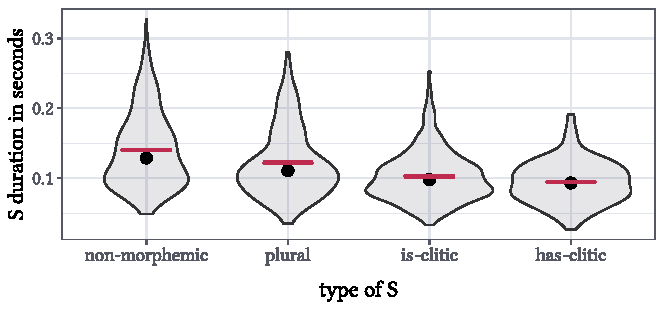
\includegraphics[]{figures/fig4.3.pdf}
    \caption{Observed durations of non-morphemic, plural, \textit{is}- and \textit{has}-clitic /s/. The dot represents the median, the horizontal line indicates the mean. The violin shapes represent rotated density plots describing the distribution of the data.}
    \label{fig:4_3}
\end{figure}

Multivariate analyses as described in the previous section were then conducted to control for the many potentially intervening influences of the described covariates listed in Section \ref{section04_2_1}. In the final model, fitted according to the procedure described above, main effects of type of /s/ (\textsc{typeOfS}), speaking rate (\textsc{speakingRate}), base duration (\textsc{baseDurLog}), pause (\textsc{pauseBin}), preceding consonant (\textsc{preC}), biphone probability sum (\textsc{biphoneProbSumBin}), following segmental type (\textsc{fol-Type}), and mono-/multilingualism (\textsc{monoMultilingual}) were found.

Regarding the random effects, only \textsc{speaker}-specific random intercepts turned out to significantly improve the model fit. The \textit{p}-values for the analysis of variance of the final model are given in Table \ref{tab:4.4}.

\begin{table}\fontsize{10}{11}
\caption{\textit{p}-values of fixed effects in the final model, fitted to the log-transformed durations of /s/.}
\label{tab:4.4}
\centering
\begin{tabular}{lrrrrrr} 
\lsptoprule
~                 & Sum Sq & Mean Sq & NumDF & DenDF   & F.value & Pr ( F)  \\ 
\midrule
\textsc{typeOfS}           & 5.312  & 1.771   & 3     & 1089.66 & 33.338  & 0.000    \\
\textsc{speakingRate}      & 0.230  & 0.230   & 1     & 1117.09 & 4.324   & 0.038    \\
\textsc{baseDurLog}        & 9.466  & 9.466   & 1     & 1079.58 & 178.220 & 0.000    \\
\textsc{pauseBin}          & 6.970  & 6.970   & 1     & 1110.28 & 131.235 & 0.000    \\
\textsc{biphoneProbSumBin} & 0.398  & 0.398   & 1     & 1082.26 & 7.492   & 0.006    \\
\textsc{preC}              & 0.623  & 0.208   & 3     & 1080.29 & 3.910   & 0.009    \\
\textsc{folType}           & 2.677  & 0.669   & 4     & 1081.55 & 12.598  & 0.000    \\
\textsc{monoMultilingual}  & 0.345  & 0.345   & 1     & 37.37   & 6.498   & 0.015    \\
\lspbottomrule
\end{tabular}
\end{table}

The final model was then analysed in terms of its R\textsuperscript{2} values which were computed with the \texttt{MuMIn} package (\cite{Barton2020}; for marginal and conditional R\textsuperscript{2} value computation, see \cite{Nakagawa2017}). The marginal R\textsuperscript{2} value of a model indicates the percentage of variation in the data explained by the fixed effects of that model. The variance explained by the entire model is given by its conditional R\textsuperscript{2} value. The marginal R\textsuperscript{2} value of the model is $0.46$, that is, fixed effects explain 46\% of the variation in the data. The variance explained by the entire model is 61\% as obtained by the conditional R\textsuperscript{2} value of $0.61$.

The estimates of the final model and their \textit{p}-values are given in Table \ref{tab:4.5}. The reference levels for the categorical predictors are: for \textsc{typeOfS} it is \texttt{non-morphemic} /s/, for \textsc{pauseBin} it is \texttt{no-pause}, for \textsc{biphoneProbSumBin} it is \texttt{low}, for \textsc{preC} it is \texttt{t}, for \textsc{folType} it is \texttt{approximant}, and for \textsc{monoMultilingual} it is \texttt{monolingual}. All coefficients can be interpreted as changes relative to these reference levels.

\begin{table}\fontsize{10}{11}
\caption{Fixed-effect coefficients and \textit{p}-values as computed by the final model (mixed-effects model fitted to the log-transformed and centred durations of /s/).}
\label{tab:4.5}
\centering
\begin{tabular}{lrrrrr} 
\lsptoprule
~                            & Estimate & SE    & df      & \textit{t}-value & Pr(\textbar{}t\textbar{})  \\ 
\midrule
(Intercept)                  & -1.321   & 0.068 & 550.378 & -19.498          & 0.000                      \\
\textsc{typeOfS}\texttt{pl}                    & -0.114   & 0.019 & 1094.00 & -6.062           & 0.000                      \\
\textsc{typeOfS}\texttt{is}                    & -0.178   & 0.020 & 1096.00 & -8.839           & 0.000                      \\
\textsc{typeOfS}\texttt{has}                   & -0.196   & 0.024 & 1091.00 & -8.140           & 0.000                      \\
\textsc{speakingRate}                 & -0.021   & 0.010 & 1117.00 & -2.079           & 0.038                      \\
\textsc{baseDurLog}                   & 0.586    & 0.044 & 1080.00 & 13.35            & 0.000                      \\
\textsc{pauseBin}\texttt{pause}                & 0.206    & 0.018 & 1110.00 & 11.456           & 0.000                      \\
\textsc{biphoneProbSumBin}\texttt{high}        & 0.047    & 0.017 & 1082.00 & 2.737            & 0.006                      \\
\textsc{preC}\texttt{f}                        & 0.061    & 0.020 & 1081.00 & -3.044           & 0.003                      \\
\textsc{preC}\texttt{k}                        & 0.055    & 0.020 & 1082.00 & -0.303           & 0.006                      \\
\textsc{preC}\texttt{p}                        & 0.050    & 0.020 & 1079.00 & 2.522            & 0.012                      \\
\textsc{folType}\texttt{F}                     & 0.012    & 0.070 & 1084.00 & 0.171            & 0.864                      \\
\textsc{folType}\texttt{N}                     & -0.036   & 0.021 & 1079.00 & -1.764           & 0.078                      \\
\textsc{folType}\texttt{P}                     & -0.045   & 0.019 & 1080.00 & -2.384           & 0.017                      \\
\textsc{folType}\texttt{V}                     & -0.136   & 0.020 & 1082.00 & -6.85            & 0.000                      \\
\textsc{monoMultilingual}\texttt{multilingual} & -0.152   & 0.059 & 37.37   & -2.549           & 0.015                      \\
\lspbottomrule
\end{tabular}
\end{table}

The predictor strength of individual predictors was checked following the method outlined in Section \ref{section03_2_1}, that is by fitting models that lacked a particular predictor and comparing their marginal R\textsuperscript{2} values to those of the final model. The results are reflected in the hierarchy given in \ref{ex:4.10}. The decrease in R\textsuperscript{2} is greatest when removing \textsc{baseDurLog}, followed by \textsc{pauseBin}, and so forth. Overall, the morphological status of an /s/ appears to be a strong predictor of its acoustic duration.

\ex.
\label{ex:4.10}
\textsc{baseDurLog >> pauseBin >> typeOfS >> monoMultilingual >> folType >> speakingRate >> biphoneProbSumBin >> PreC}

Figure \ref{fig:4_4} shows the effect of the numerical variables included in the final model on /s/ duration. The estimated values of the dependent variable and the base duration are back-transformed into seconds. Speaking rate and base duration show effects in the expected direction. With faster speech, /s/ becomes shorter (Panel A), while longer base durations also come with longer /s/ durations (Panel B). 

\begin{figure}
    \centering
    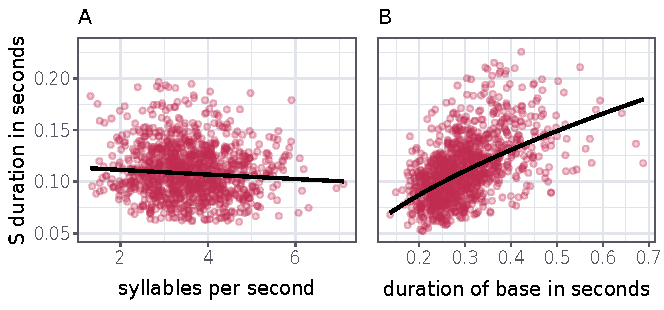
\includegraphics[width=1\textwidth]{figures/fig4.4.pdf}
    \caption{Partial effects of the numerical variables \textsc{speakingRate} (Panel A) and \textsc{baseDurLog} (back-transformed, Panel B) included in the final model, fitted to the log-transformed values of duration of /s/.}
    \label{fig:4_4}
\end{figure}


The partial effects of the categorical variables included in the final model are illustrated in Figure \ref{fig:4_5}. /s/ duration is longer if the /s/ is followed by a pause (Panel A), which can be interpreted as a clear case of phrase-final lengthening (e.g. \cite{Cooper1981}). Higher biphone probability sum leads to longer /s/ durations (Panel B). There is also an effect of the preceding consonant: The plosive /t/ is followed by significantly shorter /s/ durations than are /k/ and /f/ (Panel C). /s/ duration is significantly shorter when followed by a vowel, while all other differences between following consonants are minor in nature (Panel D). Lastly, monolingual speakers produce longer /s/ durations than multilingual speakers (Panel E).

\begin{figure}
    \centering
    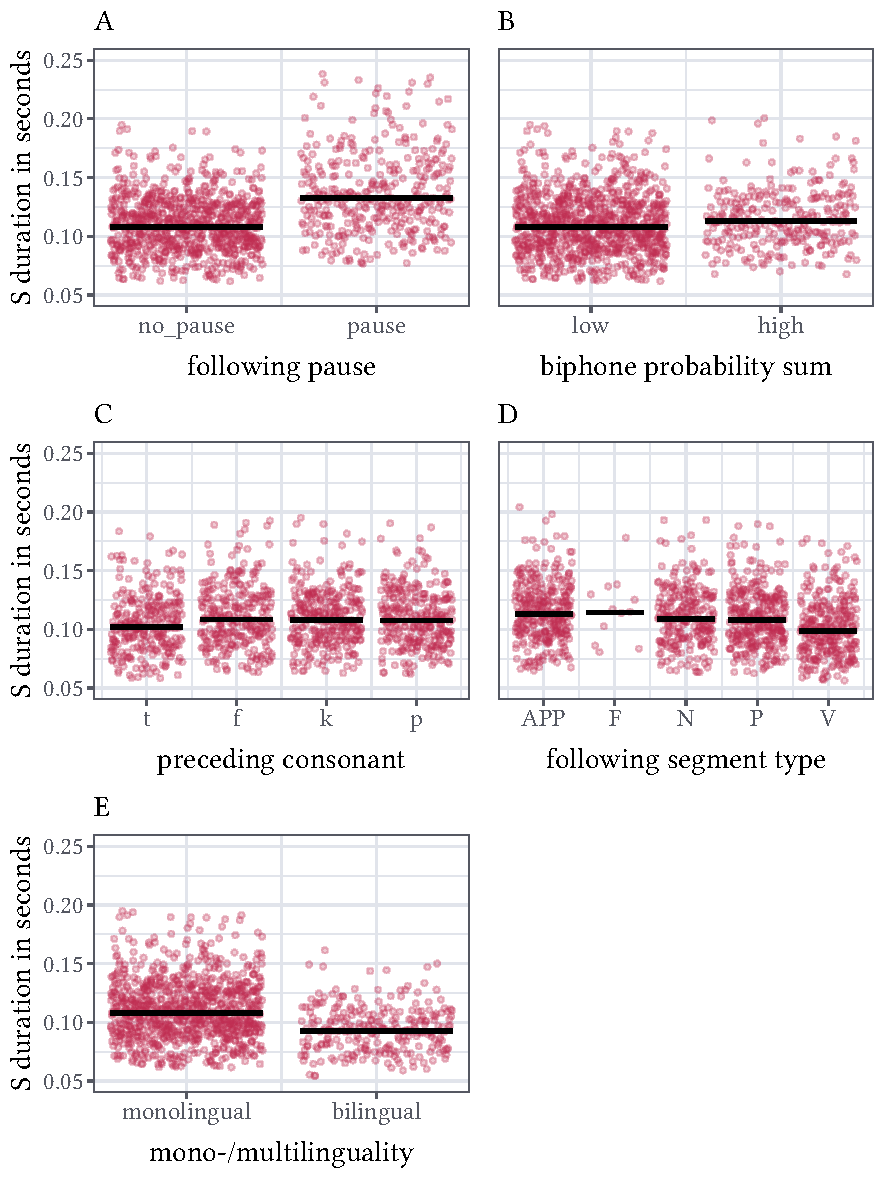
\includegraphics[]{figures/fig4.5.pdf}
    \caption{Partial effects of the categorical variables \textsc{pauseBin} (Panel A), \textsc{biphoneProbSumBin} (Panel B), \textsc{preC} (Panel C), \textsc{folType} (Panel D), and \textsc{monoMultilingual} (Panel E) included in the final model, fitted to the log-transformed values of duration of /s/.}
    \label{fig:4_5}
\end{figure}

The effect of the variable of interest, i.e. \textsc{typeOfS}, is plotted in Figure \ref{fig:4_6}. As above, the values of the dependent variable are back-transformed into seconds.

\begin{figure}
    \centering
    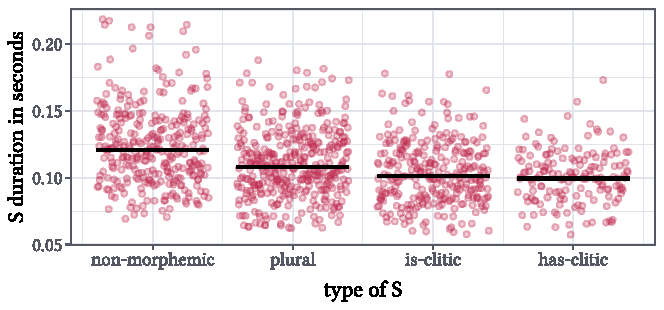
\includegraphics[width=1\textwidth]{figures/fig4.6.pdf}
    \caption{Partial effect of \textsc{typeofS} in the final model, fitted to the log-transformed values of duration of /s/.}
    \label{fig:4_6}
\end{figure}

One can see that there are durational differences between the different types of /s/. The results of pair-wise comparisons of the predicted means using Tukey contrasts (as implemented by the \texttt{SfL} package, \cite{Schmitz2021sfl}) are summarised in Table \ref{tab:4.6}.

\begin{table}\fontsize{10}{11}
\caption{Multiple comparisons of means of duration of /s/ (Tukey contrasts). Significance codes: `***' $p < 0.001$, `**' $p < 0.01$, `*' $p < 0.05$.}
\label{tab:4.6}
\centering
\begin{tabular}{llllrrrr} 
\lsptoprule
~                   & ~ & ~                  & Estimate & SE    & \textit{z}-value & Pr(\textbar{}z\textbar{}) & ~    \\ 
\midrule
plural              & - & non-morphemic      & -0.114   & 0.019 & -6.062           & 
  0.001                  & ***  \\
\textit{is}-clitic  & - & non-morphemic      & -0.188   & 0.020 & -8.839           &  0.001                    & ***  \\
\textit{has}-clitic & - & non-morphemic      & -0.196   & 0.024 & -8.140           & 
  0.001                  & ***  \\
\textit{is}-clitic  & - & plural             & -0.064   & 0.019 & -3.294           & 0.005                     & **   \\
\textit{has}-clitic & - & plural             & -0.082   & 0.023 & -3.503           & 0.003                     & **   \\
\textit{has}-clitic & - & \textit{is}-clitic & -0.018   & 0.023 & -0.766           & 0.868                     & ~    \\
\lspbottomrule
\end{tabular}
\end{table}

Based on the Tukey tests, the comparison of the different types of /s/ yields the significant contrasts shown in Table \ref{tab:4.7}. Considering the different durations given in Table \ref{tab:4.8}, the following hierarchy emerges: non-morphemic /s/ > plural /s/ > \textit{is}-/\textit{has}-clitic /s/.

\begin{table}\fontsize{10}{11}
\caption{Significant contrasts in duration between different types of /s/. Significance codes: `***' $p < 0.001$, `**' $p < 0.01$, `*' $p < 0.05$.}
\label{tab:4.7}
\centering
\begin{tabular}{lrrrr} 
\lsptoprule
~                   & nm   & pl   & \textit{is} & \textit{has}  \\ 
\midrule
non-morphemic       & n.a. & ***  & ***         & ***           \\
plural              & ~    & n.a. & **          & **            \\
\textit{is}-clitic  & ~    & ~    & n.a.        & ~             \\
\textit{has}-clitic & ~    & ~    & ~           & n.a.          \\
\lspbottomrule
\end{tabular}
\end{table}



\begin{table}\fontsize{10}{11}
\caption{/s/ durations as estimated by the final model using non-centred data. All values are back-transformed to seconds. Values given are estimated for items without following pause, high biphone sum probability, monolingual speakers, and across all preceding and following segment types.}
\label{tab:4.8}
\begin{tabular}{lr} 
\lsptoprule
\textsc{typeOfS}                      & Mean   \\ 
\midrule
non-morphemic                & 0.224  \\
plural                       & 0.200  \\
\textit{is}-clitic           & 0.187  \\
\textit{has}-clitic          & 0.184  \\
\lspbottomrule
\end{tabular}
\end{table}

To summarise, the durational differences between non-morphemic and other types of /s/, as well as the durational difference between plural and the clitics are significant, while there is no significant durational difference between the two clitics. Non-morphemic /s/ is longest in duration, followed by plural /s/, which in turn is followed by clitic /s/.

\subsection{Relative duration}\label{section04_3_2}

The results for relative duration are very similar to those of absolute duration. The \textit{p}-values for the analysis of variance of the final model are given in Table \ref{tab:4.9}. Table \ref{tab:4.10} shows the coefficients for the final model. All effects go in the same direction as in the analysis of absolute duration. The only predictors that have lost significance when compared to the model for absolute duration are \textsc{preC} and \textsc{speakingRate}. The differences in the means show the same pattern as in the analysis of absolute duration, as can be seen in Table \ref{tab:4.11}.

\begin{table}\fontsize{10}{11}
\caption{\textit{p}-values of fixed effects in the final model, fitted to the relative durations of /s/.}
\label{tab:4.9}
\centering
\begin{tabular}{lrrrrrr} 
\lsptoprule
~                 & Sum Sq & Mean Sq & NumDF & DenDF   & F.value & Pr(F)  \\ 
\midrule
\textsc{typeOfS}           & 0.161  & 0.054   & 3     & 1070.68 & 25.510  & 0.000  \\
\textsc{pauseBin}          & 0.186  & 0.186   & 1     & 1101.26 & 88.518  & 0.000  \\
\textsc{biphoneProbSumBin} & 0.015  & 0.015   & 1     & 36.32   & 6.917   & 0.012  \\
\textsc{folType}           & 0.071  & 0.018   & 4     & 1063.31 & 8.389   & 0.000  \\
\textsc{monoMultilingual}  & 0.010  & 0.010   & 1     & 37.81   & 4.561   & 0.039  \\
\lspbottomrule
\end{tabular}
\end{table}




\begin{table}\fontsize{10}{11}
\caption{Fixed-effect coefficients and \textit{p}-values as computed by the final model (mixed-effects model fitted to the relative durations of /s/).}
\label{tab:4.10}
\centering
\begin{tabular}{lrrrrr} 
\lsptoprule
~                            & Estimate & SE    & df      & \textit{t}-value & Pr(\textbar{}t\textbar{})  \\ 
\midrule
(Intercept)                  & 0.299    & 0.007 & 89.73   & 45.827           & 0.000                      \\
\textsc{typeOfS}\texttt{pl}                    & -0.019   & 0.004 & 1085.00 & -5.157           & 0.000                      \\
\textsc{typeOfS}\texttt{is}                    & -0.031   & 0.004 & 1070.00 & -7.651           & 0.000                      \\
\textsc{typeOfS}\texttt{has}                   & -0.035   & 0.005 & 1067.00 & -7.260           & 0.000                      \\
\textsc{pauseBin}\texttt{pause}                & 0.033    & 0.004 & 1101.00 & 9.408            & 0.000                      \\
\textsc{biphoneProbSumBin}\texttt{high}        & 0.013    & 0.005 & 36.32   & 2.630            & 0.012                      \\
\textsc{folType}\texttt{F}                     & 0.001    & 0.014 & 1068.00 & 0.086            & 0.931                      \\
\textsc{folType}\texttt{N}                     & -0.006   & 0.004 & 1061.00 & -1.409           & 0.159                      \\
\textsc{folType}\texttt{P}                     & -0.007   & 0.004 & 1056.00 & -1.708           & 0.088                      \\
\textsc{folType}\texttt{V}                     & -0.022   & 0.004 & 1063.00 & -5.568           & 0.000                      \\
\textsc{monoMultilingual}\texttt{multilingual} & -0.024   & 0.011 & 37.81   & -2.136           & 0.039                      \\
\lspbottomrule
\end{tabular}
\end{table}




\begin{table}\fontsize{10}{11}
\caption{Multiple comparisons of means of duration of /s/ (Tukey contrasts). Significance codes: `***' $p < 0.001$, `**' $p < 0.01$, `*' $p < 0.05$.}
\label{tab:4.11}
\centering
\begin{tabular}{lllrrrrr} 
\lsptoprule
~                   & ~ & ~                  & Estimate & SE    & \textit{z}-value & Pr(\textbar{}z\textbar{}) & ~    \\ 
\midrule
plural              & - & non-morphemic      & -0.019   & 0.004 & -5.157           & 
  0.001                  & ***  \\
\textit{is}-clitic  & - & non-morphemic      & -0.031   & 0.004 & -7.651           &  0.001                    & ***  \\
\textit{has}-clitic & - & non-morphemic      & -0.035   & 0.005 & -7.260           & 
  0.001                  & ***  \\
\textit{is}-clitic  & - & plural             & -0.011   & 0.004 & -2.936           & 0.017                     & *    \\
\textit{has}-clitic & - & plural             & -0.015   & 0.005 & -3.300           & 0.005                     & **   \\
\textit{has}-clitic & - & \textit{is}-clitic & -0.004   & 0.005 & -0.854           & 0.827                     & ~    \\
\lspbottomrule
\end{tabular}
\end{table}



\section{Discussion}\label{section04_4}

Following in the footsteps of previous studies on durational differences between different types of /s/, this study tested whether the morphological category of word-final /s/ has an influence on its acoustic duration in speech production. In order to avoid imbalanced data as in the case of corpus studies, speech material elicited by the means of highly controlled contexts of a production task was used. For the first time in this context, pseudowords instead of real words were used to minimise potentially confounding lexical effects. It was found that there are significant durational differences between non-morphemic and morphemic types of word-final /s/, with morphemic types of /s/ being significantly shorter in duration than non-morphemic /s/. Also, there are significant durational differences between the plural suffix and the \textit{is}- and \textit{has}-clitic /s/, with plural /s/ being significantly longer than clitic /s/ and with no significant difference between the two clitics. Hence, the type of /s/ emerged as a strong, significant predictor of segmental duration.

The differences between different types of /s/ in the present study are completely in line with previous studies that were based on speech corpora and on different varieties of English (\cite{Plag2017} and \cite{Tomaschek2019} on North American English; \cite{Zimmermann2016} on New Zealand English). In those studies the same pattern of differences was found. Turning to previous experimental studies, differing results are found. The results of both prior experimental studies (\cite{Walsh1983, Seyfarth2017}) are subject to potentially confounding effects of the lexical and contextual properties of the items under investigation. Their finding of non-morphemic /s/ being shorter than morphemic /s/ may well be an artefact of such properties. The items used in the present study, however, are much less prone to be subject to such effects as they are pseudowords with no established representations in the speakers’ mental lexicons. The results on the duration of clitic /s/ cannot be compared to previously reported ones by other experimental studies, as none of the previously conducted experimental studies investigated clitic /s/ production.

No previous studies have used pseudowords either, so before turning to the theoretical interpretation of the results of the present study, a few words are in order on whether using pseudowords might have had an undesired impact on the results. While the use of pseudowords in phonetic experiments comes with a number of benefits (see Section \ref{section03_1_1}), it also raises some questions. First, there is the issue of phonotactic probability raised in Section \ref{section04_2_1}. Two measures concerned with phonotactics (one describing the phonotactic probability of the whole word, the other taking into consideration the consonant preceding the word-final /s/) were included in the statistical analysis to address this issue. It turned out that phonotactic probability influences the production of pseudowords, as it does for real words. Crucially, there was no interaction between the type of /s/ and the consonant preceding it in mono-morphemic words. This means that speakers produced these clusters in the same way, no matter whether the cluster occurred in the mono-morphemic words or whether the cluster straddled the morphemic boundary between the base and the /s/. The main effects of the phonotactic variables turned out to be rather weak and, crucially, were properly controlled for in the regression analysis. In sum, the phonotactics of the final cluster does not seem to have unduly influenced the results.

Second, there might have been a problem with another aspect of the phonological structure of the pseudowords in the experiment, i.e. long-distance agreement of phonological features (\cite{Coetzee2009}). Such effects of the Obligatory Contour Principle (OCP; \cite{Coetzee2005}) might have arisen with pseudowords such as \textit{pleep} (in which initial /p/ and final /p/ share all features) or \textit{glik} (in which the initial and final sounds /g/ and /k/ share the dorsal feature). Following the findings by \citet{Coetzee2009}, a new variable was coded to test this effect post-hoc as an additional covariate and as an interacting term of \textsc{typeOfS} with the following levels: \texttt{not well-formed} for pseudowords in which the initial and final consonant share all features (n = 836), \texttt{moderately well-formed} for pseudowords in which the initial and final consonant share the dorsal feature (n = 147), and \texttt{well-formed} for all remaining pseudowords (n = 145). There was no significant main effect of this variable on the duration of /s/, nor a significant interaction with \textsc{typeOfS}. OCP effects thus cannot explain the present results.

Third, after having carried out the experiments, it came to attention that some of the pseudowords have real word relatives that are spelled differently but are phonologically identical:  \textit{pleet(s)} corresponds to \textit{pleat(s)}, \textit{glits} corresponds to \textit{glitz} (and no word corresponding to \textit{glit}), and \textit{glik} corresponds to the surname \textit{Glick} (and no surname corresponding to \textit{gliks}), whereas \textit{glif(s)} corresponds to \textit{glyph(s)}, which has a very low frequency and thus may constitute a pseudoword for most of the participants. These words might have unduly influenced the results and should perhaps not have been included into the statistical analysis. To check whether these items had any influence on the results, a data set was created containing all data but the four potentially offending items. Fitting the final model (as done in Section \ref{section04_2_4}) to this new dataset resulted in basically the same findings, i.e. \textsc{typeOfS} was still a significant predictor for /s/ duration showing the same significant differences between non-morphemic, plural, and clitic items as presented in Table \ref{tab:4.7}.

It has recently been shown that the notion of pseudoword is problematic in a more general way (also see Section \ref{section03_1_1}). The notion of pseudoword itself is usually based on the idea of the lexicon as a community construct. When talking about the mental lexicon, however, it is clear that what is an existing word and what is an unknown pseudoword is a matter of the individual speaker’s mental lexicon. All participants of the present experiment denied knowing any of the pseudowords used in this experiment when asked afterwards. At the community level, Google frequencies of pseudowords have been shown to be a robust predictor of reaction times in lexical decision tasks (e.g. \cite{Hendrix2020}). To test whether Google frequency had an effect on the present results, the covariate \textsc{googleFreq} was created containing the number of Google search hits for each pseudoword. The addition of this covariate as either fixed effect or interacting term to \textsc{typeOfS} resulted in its exclusion during the model simplification procedure.

Finally, let us turn to the theoretical implications of the present results. What do these results mean for the three hypotheses that were tested? \textsc{H prod\textsubscript{1}}, the ``Feed-Forward Hypothesis", states that there is no durational difference between word-final non-morphemic /s/, plural /s/, and auxiliary clitic /s/. This hypothesis is rejected as carefully controlled evidence was provided that shows that the duration of /s/ varies by morphological category. This is an effect that present feed-forward models cannot accommodate, unless they would be refined in such a way that post-lexical processes can arise from certain kinds of lexical information. At present, no such refinement is available. 

\textsc{H prod\textsubscript{2}}, the ``Prosodic Hypothesis", states that there are durational differences between different types of word-final /s/, with non-morphemic /s/ being shorter than plural /s/, and plural /s/ being shorter than the auxiliary clitic. While it is true that there are durational differences between the categories, the observed differences pattern in the opposite direction. The more integrated the /s/ is with the stem, the longer its duration. The ``Prosodic Hypothesis" is correct in positing that the two auxiliary clitics should show no difference in duration. Overall, however, the ``Prosodic Hypothesis" must be rejected, as the prosodic structure does not explain the most important patterning of the data.

Finally, \textsc{H prod\textsubscript{3}}, the ``Emergence Hypothesis", states that there are durational differences between the different types of word-final /s/ under investigation. The fact that such differences were found means that these differences might emerge through the mechanisms posited by the theories underlying this hypothesis. 

As mentioned in Section \ref{section02_1}, \citet{Tomaschek2019} found that stronger support for a morphological function leads to a longer duration, that is as for our findings, non-morphemic /s/ showed the longest duration, auxiliary clitic /s/ showed the shortest durations, and plural suffix /s/ duration was in between. This effect seems to run counter to the predictions of information-theoretic accounts and probabilistic theories, according to which words and segments are realised shorter when they are less informative (\cite{Aylett2004,Jaeger2010,Priva2015}). However, the enhancement effects are in line with studies showing that duration increases with increasing paradigmatic certainty (\cite{Kuperman2007, Cohen2014, Bell2021, Tucker2019Sims}). For instance, \citet{Kuperman2007} found that the duration of a given interfix in Dutch compounds increases with increasing probability of this interfix (as against its competitors) in the left constituent family of the compound. 

Overall, it seems that simplistic approaches can neither explain the existence, nor the patterning of the durational differences one finds attested. The ``Feed-Forward Hypothesis" is rejected because durational differences were in fact observed. The ``Prosodic Hypothesis" is rejected because the observed durational differences pattern in a direction that is opposite to the one predicted. The ``Emergence Hypothesis" is supported by the present findings as it proposes that durational differences of some nature should emerge between different types of /s/.

The results of the present study may bring up further questions. First, how can the aforementioned effects of morphological support, informativity, and paradigmatic probability be reconciled? This question is addressed further in Chapter \ref{chapter05}, making use of linear discriminative learning (\cite{Baayen2019, Chuang2021}). Second, assuming the durational differences found here and in previous studies are indeed systematic, one would also like to know whether language users are able to perceive them. This automatically leads to the question of whether all differences are perceptible or only some of them, given our knowledge on the perception of differences in fricative durations, i.e. that the threshold for perceptible durational differences appears to be at 25 ms (\cite{Klatt1975}). This question is further investigated in Chapter \ref{chapter06}. Third, if the durational differences are perceptible, another question naturally suggests itself: Do users of a language not only perceive but also make use of such differences in comprehension? This question is addressed in Chapters \ref{chapter07} and \ref{chapter08}.
